\documentclass[sigconf]{acmart}

% Disable / remove copyright boxes
\setcopyright{none}
\settopmatter{printacmref=false}
\renewcommand\footnotetextcopyrightpermission[1]{}

% Increase margin between text and footer
\setlength{\footskip}{20pt}

% Add CCR footer
\usepackage{fancyhdr}
\fancypagestyle{plain}{%
   \fancyhf{} %
   \fancyfoot[L]{Master Practical Course: Internet Measurements and Reproducibility Lab}%
   \fancyfoot[R]{Winter Semester 2020/21}%
}
\pagestyle{plain}

% Add CCR footer on first page
\fancypagestyle{firstpagestyle}{%
   \fancyhf{} %
   \fancyfoot[L]{Internet Measurements and Reproducibility Lab}%
   \fancyfoot[R]{Winter Semester 2020/21}%
}

% Add editorial note
%\begin{teaserfigure}
%	\parbox{\textwidth}{\centering\normalsize
%		This article is an editorial note submitted to CCR. It has NOT been peer reviewed.\\
%		The authors take full responsibility for this article's
%		technical content. Comments can be posted through CCR Online.
%	}
%	\vspace{10pt}
%\end{teaserfigure}

\usepackage{balance}
\usepackage{subcaption}

\begin{document}

\title{Reproducibility Report: Web Performance Pitfalls}

\author{Curt Polack}
\affiliation{
	\institution{TU Munich, Germany}
}
\email{curt.polack@tum.de}

\begin{abstract}
	In this paper, we re-implement a work published in proceedings of the 20th International Conference for Passive and Active Measurement (PAM) in 2019: ``Web Performance Pitfalls''. The paper used a number of web-scraping and performance evaluation tools to perform measurements of ca. 2000 popular websites. These measurements were used to demonstrate and evaluate differences in measurements by tool, standard, etc. that can cause different and possibly misleading results in papers that examine web performance.
	
	This paper details the process of reproducing the original results and conclusions using the data and scripts provided in the original paper. It also details the use of the aforementioned scripts to perform a new set of measurements for ca. 1000 popular websites. The difficulties of obtaining new measurements and their results are expounded upon and the results compared with those of the original paper.
	
	The original data provided produced results that coincide with the results and plots in the original paper. The measurement scripts provided for Chrome and Firefox with Selenium did not work in either the environment used in the original paper or in a modern Linux environment. The measurements that were collected using Firefox with Marionette and analyzed by the scripts provided did, however, generate similar results to those produced by the original data regarding two major web performance metrics: load time and number of objects. The new measurement's results did not correspond to those of the original dataset regarding object counts. 
\end{abstract}

\begin{CCSXML}
<ccs2012>
	<concept>
	<concept_id>10003033.10003079</concept_id>
	<concept_desc>Networks~Network performance evaluation</concept_desc>
	<concept_significance>500</concept_significance>
	</concept>
</ccs2012>
\end{CCSXML}

\begin{CCSXML}
<ccs2012>
	<concept>
	<concept_id>10003033.10003079.10011704</concept_id>
	<concept_desc>Networks~Network measurement</concept_desc>
	<concept_significance>500</concept_significance>
	</concept>
</ccs2012>
\end{CCSXML}

\ccsdesc[500]{Networks~Network performance evaluation}
\ccsdesc[500]{Networks~Network measurement}

\keywords{Web performance, Measurement}

\maketitle

\section{Motivation \& Summary of Original Paper}

\begin{frame}
    \frametitle{Motivation}
    A number of metrics have been developed and used as benchmarks to accurately reflect the performance of web applications for users. \textbf{Measurements can differ greatly depending on a number of factors:}
    \begin{itemize}
        \item Surveyed Web Pages
        \item User Devices
        \item Browsers
        \item Tools (e.g. Selenium)
        \item Metrics
    \end{itemize}
    $\boldsymbol{\rightarrow}$ This diversity as well as the lack of clearly established standards lead to difficulties when quantifying performance. The original paper \cite{10.1007/978-3-030-15986-3_19} examined the effects of these ambiguities with regards to browsers, tools, and metrics and provided guidelines for future papers.
\end{frame}

\begin{frame}
    \frametitle{Summary of Original Paper}
	The original paper \cite{10.1007/978-3-030-15986-3_19} was structured as follows:
    \begin{enumerate}
        \item Introduction
        \item Metric Definitions \& Tools
        \item Survey of 15 Web Studies
        \item Methodology
        \item Identification of Pitfalls \& Guidelines for Future Papers
    \end{enumerate}
\end{frame}
\section{Background}
\label{sec:background}
Among the most important web metrics are load times, number \& size of objects, and page size. Each of the aforementioned metrics can be measured according to numerous definitions and using data from diverse data sources. The following section provides an overview of these definitions and the data sources used in this paper.

\subsection{Load Times}
The time required for loading a web page correlates strongly with user experience \cite{6263888}. A browser normally loads a web page in multiple steps: load and parse the base document, construct a Document Object Model (DOM), load and process referenced objects, render / display the results. Although Page Load Time (PLT), defined as the time until the onLoad event, is most often used to measure page load times, there are a number of other metrics. For example, Time To First Paint (TTFP) and Above The Fold Time (AFT) are triggered before PLT when the content is first displayed and available to the user. The start times used for calculating load times can always differ (e.g. navigationStart, fetchStart). One of the main takeaways from \cite{10.1007/978-3-030-15986-3_19} is that redirects can strongly affect these measurements and should be accounted for; Figure \ref{fig:plot_redirects} shows the impact redirects can have on PLT and Figure \ref{fig:bar_redirects} the prevalence of such redirects. 

There is also a plurality of data sources for calculating load times. The standardized API for navigation timings \cite{timing_2012} is used to fetch load times based on browser events. It is important to note that events / metrics provided by the Navigation Timings API are not necessarily defined in the same way for all browsers. HTTP Archive files \cite{har_format_2012} and the Resource Timings API \cite{w3c_2020} also provide load time data. The majority of modern browsers (e.g. Chrome, Firefox) implement the Navigation Timings and Resource Timings APIs; HAR files can be exported using developer tools. Both Chrome and Firefox provide remote debugging and page load automation interfaces (i.e. Chrome DevTools \& Firefox Marionette). There are also third-party automation frameworks that allow for the same basic functionality as well as extended functions (e.g. keyboard input); Selenium, one of the most popular such tools, is used in the original paper.

 \begin{figure}
 \centering
 \begin{subfigure}{\linewidth}
		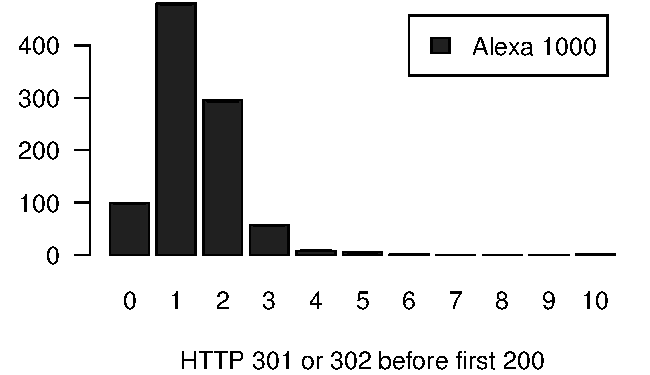
\includegraphics[width=\linewidth]{New_Plots/barplot_redirects_clean.pdf}
	\caption{New Measurements}
	\label{fig:new_bar_redirects}
\end{subfigure}\par\medskip
\begin{subfigure}{\linewidth}
		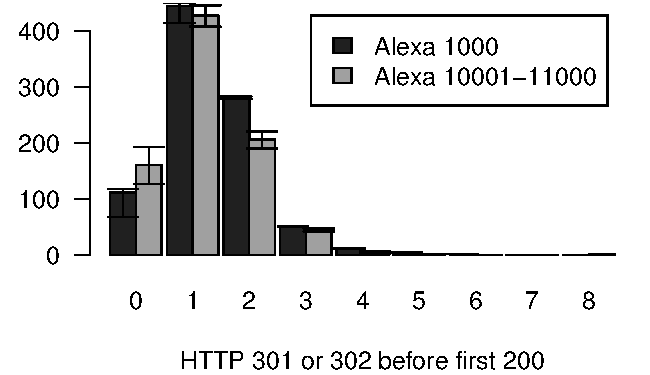
\includegraphics[width=\linewidth]{Original Plots/barplot_redirects.pdf}
	\caption{Original Measurements}
	\label{fig:orig_bar_redirects}
\end{subfigure}
\caption{Number of initial Redirects}
\label{fig:bar_redirects}
\end{figure}

\begin{figure}
 \centering
 \begin{subfigure}{\linewidth}
		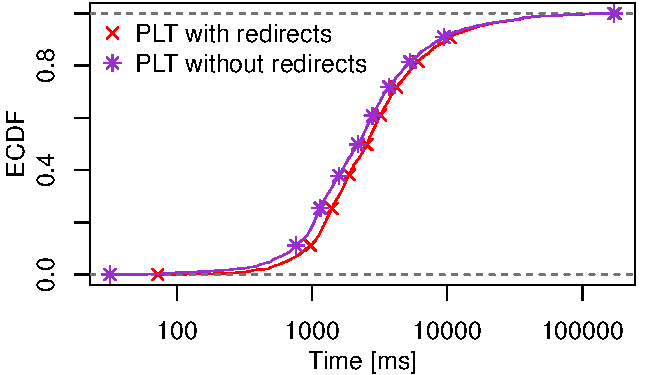
\includegraphics[width=\linewidth]{New_Plots/ecdf_loadtimes.pdf}
	\caption{New Measurements}
	\label{fig:new_plot_redirects}
\end{subfigure}\par\medskip
\begin{subfigure}{\linewidth}
		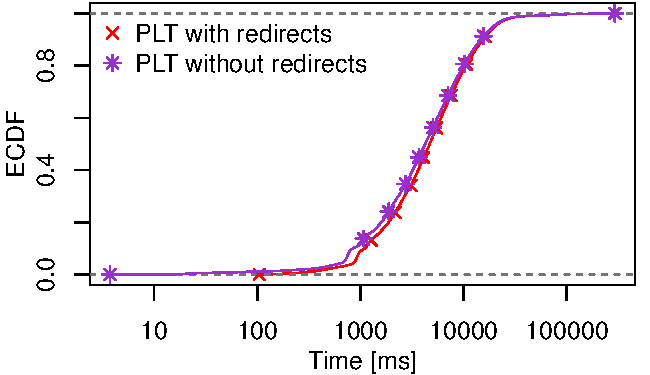
\includegraphics[width=\linewidth]{Original Plots/ecdf_loadtimes.pdf}
	\caption{Original Measurements}
	\label{fig:orig_plot_redirects}
\end{subfigure}
\caption{Page Load Time (PLT) with and without initial redirects}
\label{fig:plot_redirects}
\end{figure}

\subsection{Number and Size of Objects}
In order to estimate the complexity of web pages, metrics such as Object Index, Object Count, and Byte Index are employed. Since web pages are often constantly loading - even after the initial page load - object counts should only count objects loaded by the onLoad event. Calculating a count of the initial objects can be done using objects in the DOM or HTTP request-response pairs. Object size normally reflects the encoded size (i.e. the count of bytes transferred over the network) but can also reflect the decoded (i.e. decompressed) number of bytes. Byte Index refers to the integral of the total sizes of objects loaded over time and is an important metric for the size of Objects \cite{10.1145/2940136.2940138}.

To obtain the number of objects, one can count the number of HTTP request-response pairs in HAR files. The number of objects can also be obtained using the Resource Timings API. Both the Resource Timings API and HAR files supply the encoded and decoded body size. Alternatively, the number of objects can be extracted from packet capture traces if all elements can be decrypted; if this is not the case, object sizes can differ due to TLS padding.
\section{Experimental Setup \& Re-implementation}
\label{sec:reimplement}
This section details the experimental setup used both in the original paper \cite{10.1007/978-3-030-15986-3_19} as well as this paper. It also documents the process of and difficulties during the data collection and evaluation. Lastly, it describes the origins of the datasets used.

\subsection{Experimental Setup}
\citeauthor{10.1007/978-3-030-15986-3_19} used the following tools: (1) Firefox 61.0.2 with Selenium 3.14.0 and geckodriver 0.21.0, (2) Firefox 62.0.2 with Marionette, and (3) Chrome 69 with Chrome DevTools. This multitude of tools was used in order to provide data for a comparison of different frameworks as well as web pages. All pages were loaded on a Thinkpad L450 running Debian 9 (Stretch). The extension used to export HAR files was har-export-trigger 0.6.1. The Thinkpad (i.e. vantage point) was connected directly to a university network to avoid bandwidth / latency issues. To minimize the effects of DNS caching and resolver delay, a recursive resolver within close range (in terms of the network) was used. 

The hardware and software employed in this paper were similar yet more modern. Ubuntu 20.04. was run in a virtual machine on a Matebook X Pro (1st Generation). The use of the following tools was attempted / responsible for the results: (1) Firefox 82 with Selenium 3.141.59 and geckodriver 0.29.0, (2) Firefox 82 with Marionette, and (3) Chrome 88 with Chrome DevTools. The extension used to export HAR files was, as in the original version, har-export-trigger 0.6.1. as no new versions were released since the original paper. The vantage point was connected directly to a stable home network using ethernet; the connection was not shared for the duration of the tests. A recursive DNS resolver close to the vantage point, in terms of the network, was used as well. During testing of scripts in the new environment, there were difficulties; a second virtual machine with the original experimental setup (Debian Stretch, etc.) was used to reproduce / solve these issues. Despite trying the versions specified in the original paper as well as the more modern versions, it was not possible to consistently extract HAR files using Firefox with Selenium and Chrome with PyDevTools as specified in the original paper. 

\subsection{Scripts}
\label{sec:scripts}
All scripts used in \cite{10.1007/978-3-030-15986-3_19} are available in \cite{enghardt_2019}. The scripts are grouped into three categories: measurement / load, computation, and evaluation. The measurement scripts include separate scripts for each of the aforementioned tools (e.g. Firefox with Selenium) as well as a script to parse the exported data and capture packets for comparison with and verification of the results. The computation scripts take the raw results as input and output standardized data that is then used by the evaluation scripts to provide percentiles, averages, and graphs.

The scripts for Firefox with Selenium and Chrome with DevTools were unable to export HAR files in both the Ubuntu virtual machine with all updates installed or a Debian virtual machine using the software versions specified in the original paper. The inability to export the HAR files that were key to the measurements which compared tools led to the decision to focus on reproducing measurements using Firefox with Marionette; this decision meant that results for chrome could not be reproduced. Multiple of the computation and evaluation scripts also exhibited a number of smaller errors, e.g. the compute script was not compatible with the original data format. The adjusted / corrected scripts are available in the following on GitHub\footnote{\url{https://github.com/curtp67/web-measurement-tools-reproduction}}.

\subsection{Datasets}
Alexa Top Lists are, despite some well-known limitations, among the most used data sources for research regarding the internet \cite{10.1145/3278532.3278574}. For this reason, \citeauthor{10.1007/978-3-030-15986-3_19}  used two distinct website lists in their paper: Alexa 1000 (September 18, 2018) and Alexa 10001-11000 (September 30, 2018). Each page was accessed a total of 10 times using different framework over a period of several days. In this paper, I used Alexa 1000 (January 18, 2021) and performed 3 measurements for each website over a period of several days. The original\footnote{\url{http://dx.doi.org/10.14279/depositonce-8100}} and reproduced\footnote{\url{https://syncandshare.lrz.de/getlink/fiFSuxPcpDVkZhwfeTVNDYxc}} datasets collected can be found online. The captured packets (pcap format) that were used to verify results were also not available in the original dataset due to their size.

\begin{figure}[ht!]
		\centering
\begin{subfigure}{\linewidth}
		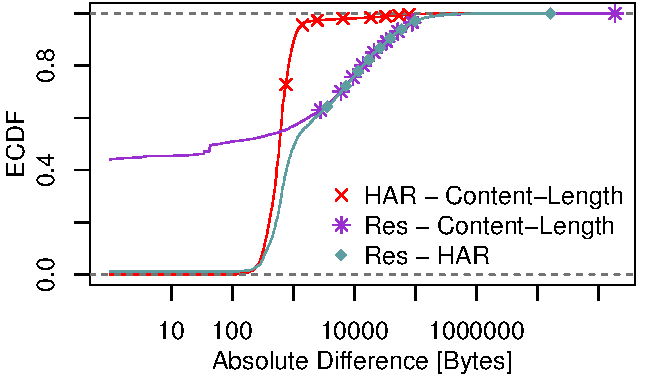
\includegraphics[width=\linewidth]{New_Plots/ecdf_diff_objectsizes.pdf}
	\caption{New Measurements}
	\label{fig:new_absolute_byte_index}
\end{subfigure}\par\medskip
 \begin{subfigure}{\linewidth}
		\centering
		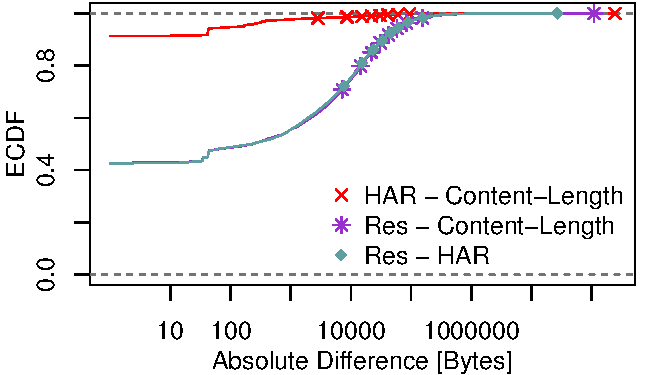
\includegraphics[width=\linewidth]{Firefox Plots/ecdf_diff_objectsizes.pdf}
	\caption{Original Measurements (Firefox Only)}
	\label{fig:orig_absolute_byte_index}
\end{subfigure}
 \begin{subfigure}{\linewidth}
		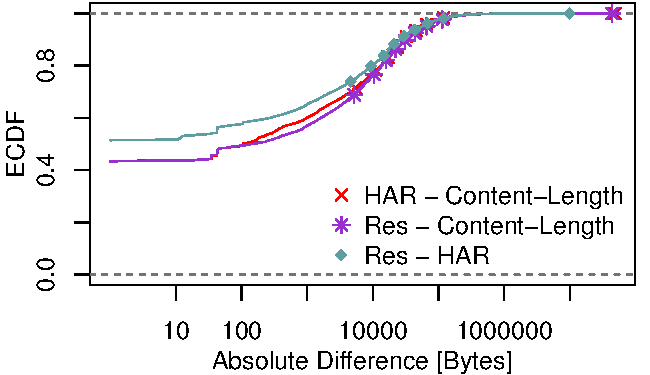
\includegraphics[width=\linewidth]{Chrome_Plots/ecdf_diff_objectsizes.pdf}
	\caption{Original Measurements (Chrome Only)}
	\label{fig:orig_chrome_absolute_byte_index}
\end{subfigure}
\caption{Object sizes: differences due to metric for all objects}
	\label{fig:absolute_byte_index}
\end{figure}
%\section{Datasets}
The increasing dependence on fast, reliable networks in academia and elsewhere necessitated the formalization of those networks. Quality of Service (QoS) guarantees regarding delay, throughput, and packet loss are especially important when measuring the performance of networks and ensuring their QoS \cite{10.1007/978-3-030-15986-3_19}.
\section{Evaluation}
In their original work, \citeauthor{10.1007/978-3-030-15986-3_19} identified four pitfalls and their effects in the collected datasets. This section examines three major pitfalls: Redirects, Object Sizes, and Byte Index more closely using both data from the original dataset and the newly collected measurements. 

\subsection{Redirects}
As mentioned in Section \ref{sec:background}, \citeauthor{10.1007/978-3-030-15986-3_19} makes the observation that initial redirects can increase PLT substantially. As seen in Figure \ref{fig:plot_redirects}, the dataset provided in the original paper also makes the more specific observation that this effect is especially pronounced for short page loads. While the new measurements / dataset does confirm that initial redirects can have a large effect on PLT, the difference in short load times is less pronounced. 

The percentage of redirects taking an abnormally long time remained relatively constant between both datasets: In the original dataset, 11.20482\% (Firefox Datasets Only: 13.9249\%) of redirects take more than one second; The new dataset provides a similar result with 12.34043\% of redirects taking more than one second. The number of redirects increased slightly in the new dataset: in the original dataset, the mean number of redirects in measurements performed by Firefox using Marionette was 1.258; the new dataset's measurements produced a mean number of redirects of 1.393. The new dataset confirms that redirects can have an impact on PLT, albeit less significant than in the original dataset. The suggestion for papers to make a conscious choice regarding the inclusion or exclusion of redirects in timing is, therefore, still valid.

\subsection{Object Sizes}
In the original paper, \citeauthor{10.1007/978-3-030-15986-3_19} compare the object sizes for all pages (including those transferred over encrypted connections). In Figure \ref{fig:relative_byte_index}, the object size differences across the different data sources (HAR file body size, Content-Length header in HAR file, and Resource Timings) are displayed. Content-Length header (taken from browser) is used as a close approximation for a baseline. In the original dataset (Firefox Only): Resource timings, HAR body size, and HAR Content-Length provide the exact same object size as the baseline in 42.5\%, 91.3\%, 42.4\% of cases respectively. These percentages are drastically different in the new dataset for both HAR body size and HAR Content-Length: Only 0.02\% and 0.88\% match the baseline exactly. Resource Timings, however, provide a relatively accurate measure of object sizes and math the baseline in 43.88\% of all cases.

This data, as shown in Figure \ref{fig:absolute_byte_index}, clearly shows that the new measurements do not confirm the conclusion that Content-Length found in HAR files is the most accurate measure of object sizes. The new dataset instead leads to the conclusion that object sizes provided by Resource Timings provide the most accurate approximation of total object size. The fact that it is only an exact match in fewer than half of all cases, however, does not make it an ideal measure. The difference between HAR Content-Length is very strongly concentrated in one range between 100 and 1000 bytes, where over 90\% of measurements can be found (see Figure \ref{fig:new_absolute_byte_index}); this suggests that there is a consistent reason for this difference and that it can be accounted for (e.g. with a constant offset). 

\begin{figure}
 \centering
 \begin{subfigure}{\linewidth}
		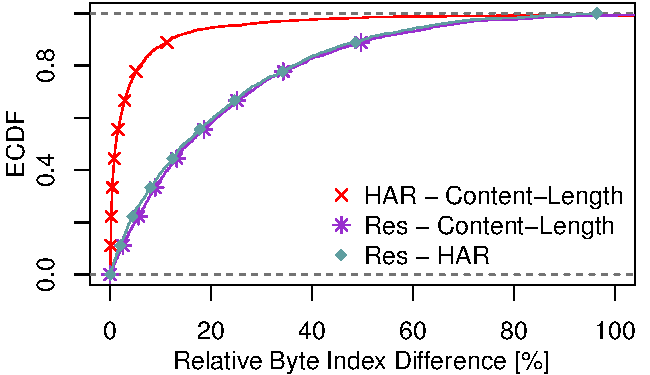
\includegraphics[width=\linewidth]{New_Plots/ecdf_rel_object_byte_index.pdf}
	\caption{New Measurements}
	\label{fig:new_relative_byte_index}
\end{subfigure}\par\medskip
 \begin{subfigure}{\linewidth}
		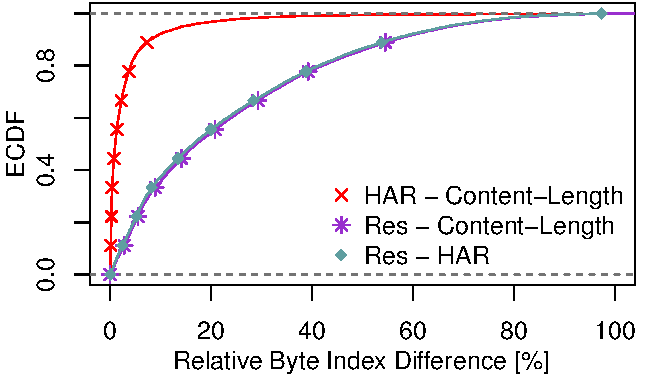
\includegraphics[width=\linewidth]{Firefox Plots/ecdf_rel_object_byte_index.pdf}
	\caption{Original Measurements (Firefox Only)}
	\label{fig:orig_firefox_relative_byte_index}
\end{subfigure}\par\medskip
 \begin{subfigure}{\linewidth}
		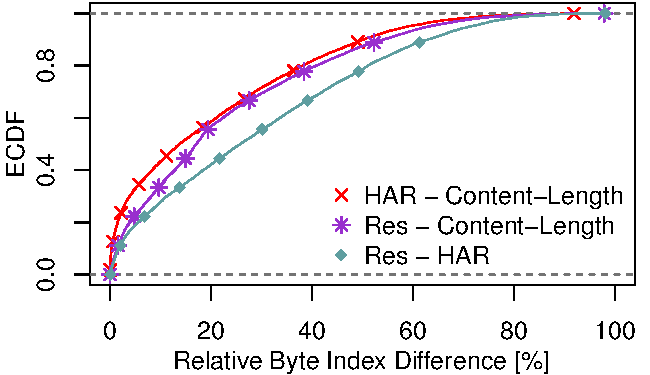
\includegraphics[width=\linewidth]{Chrome_Plots/ecdf_rel_object_byte_index.pdf}
	\caption{Original Measurements (Chrome Only)}
	\label{fig:orig_chrome_relative_byte_index}
\end{subfigure}
\caption{Byte index: difference due to data source}
\label{fig:relative_byte_index}
\end{figure}

\subsection{Object Count \& Byte Index}
In the original paper, \citeauthor{10.1007/978-3-030-15986-3_19} found that not only do object sizes differ significantly by data source but also object counts. In the original Alexa 1000 dataset, object counts for the same web pages differed between HAR files and Resource Timings by at least 7 objects. Figure \ref{fig:relative_byte_index} shows the relative difference between Byte Index for the same page load using HAR body size, Resource Timings body size and the Content Length header. As observed in the original measurements (Firefox Only), the Byte Index is close to identical for Content-Length and HAR body size; this observation is confirmed in the new measurements, as seen in Figure \ref{fig:new_relative_byte_index}. 

The results for Chrome, as seen in Figure \ref{fig:orig_chrome_relative_byte_index}, show that the Byte Index for both Resource Timings and HAR differed significantly from that of Content-Length. Unfortunately, due to the difficulties described in \ref{sec:scripts} it was not possible to confirm these findings using new measurements in Chrome. Thus, the conclusion of the original paper that resource timings do not include all objects of a web page is confirmed by the new dataset for Firefox.
\section{Conclusion}
In this paper, we re-implemented the paper Web Performance Pitfalls, published in 2019 during the International Conference for Passive and Active Measurement (PAM). The re-implementation focused on reproducing the conclusions of the original paper using the data provided publicly as well as taking new measurements to confirm it. During the implementation process, problems with a number of the provided scripts caused smaller adjustments to be necessary and no measurements to be taken with 2/3 of the frameworks (i.e. Firefox with Selenium and Chrome with DevTools). Three new datasets were created using the scripts, based on the Alexa 1000 list.

This paper's reproduction effort focused mainly on three main pitfalls that were described in the original paper: Redirects, Object Size, and Object Count. The results required for the conclusions drawn for these pitfalls were confirmed by the original data, but only 2 / 3 were confirmed by the new measurements created using Firefox with Marionette on a modern system. The new dataset contradicts the conclusion in the original paper that the Content-Length in HAR files is the most reliable data source for object sizes but does confirm the large inconsistencies in object size between data sources. The other examined conclusions regarding redirects and object count / byte index were confirmed by the new dataset.

The plots and results found in this work and the original paper can be reproduced using the data and scripts available online, as described in Section \ref{sec:reimplement}. The data in both papers underlines the importance of improving the documentation of studies of web performance as well as choosing performance metrics carefully and deliberately.

%\begin{acks}
%	The discussions leading to this editorial were initiated during
%	Dagstuhl Seminar 15102 on
%	\emph{Secure Routing for Future Communication Networks},
%	and we thank all participants for their contributions.
%\end{acks}

{ \balance
{
	\bibliographystyle{ACM-Reference-Format}
	%\bibliography{literature}
\bibliography{paper}
}
}

\end{document}
